%%%%%%%%%%%%%%%%%%%%%%%%%%%%%%%%%%%%%%%%%
% Jacobs Landscape Poster
% LaTeX Template
% Version 1.1 (14/06/14)
%
% Created by:
% Computational Physics and Biophysics Group, Jacobs University
% https://teamwork.jacobs-university.de:8443/confluence/display/CoPandBiG/LaTeX+Poster
% 
% Further modified by:
% Nathaniel Johnston (nathaniel@njohnston.ca)
%
% This template has been downloaded from:
% http://www.LaTeXTemplates.com
%
% License:
% CC BY-NC-SA 3.0 (http://creativecommons.org/licenses/by-nc-sa/3.0/)
%
%%%%%%%%%%%%%%%%%%%%%%%%%%%%%%%%%%%%%%%%%

%----------------------------------------------------------------------------------------
%	PACKAGES AND OTHER DOCUMENT CONFIGURATIONS
%----------------------------------------------------------------------------------------

\documentclass[final]{beamer}

\usepackage[scale=1.33]{beamerposter} % Use the beamerposter package for laying out the poster

\usetheme{confposter} % Use the confposter theme supplied with this template

\setbeamercolor{block title}{fg=dblue!70,bg=white} % Colors of the block titles
\setbeamercolor{block body}{fg=black,bg=white} % Colors of the body of blocks
\setbeamercolor{block alerted title}{fg=white,bg=dblue!70} % Colors of the highlighted block titles
\setbeamercolor{block alerted body}{fg=black,bg=dblue!10} % Colors of the body of highlighted blocks
% Many more colors are available for use in beamerthemeconfposter.sty

%-----------------------------------------------------------
% Define the column widths and overall poster size
% To set effective sepwid, onecolwid and twocolwid values, first choose how many columns you want and how much separation you want between columns
% In this template, the separation width chosen is 0.024 of the paper width and a 4-column layout
% onecolwid should therefore be (1-(# of columns+1)*sepwid)/# of columns e.g. (1-(4+1)*0.024)/4 = 0.22
% Set twocolwid to be (2*onecolwid)+sepwid = 0.464
% Set threecolwid to be (3*onecolwid)+2*sepwid = 0.708

\newlength{\sepwid}
\newlength{\onecolwid}
\newlength{\twocolwid}
\newlength{\threecolwid}
\setlength{\paperwidth}{48in} % A0 width: 46.8in
\setlength{\paperheight}{36in} % A0 height: 33.1in
\setlength{\sepwid}{0.024\paperwidth} % Separation width (white space) between columns
\setlength{\onecolwid}{0.22\paperwidth} % Width of one column
\setlength{\twocolwid}{0.464\paperwidth} % Width of two columns
\setlength{\threecolwid}{0.708\paperwidth} % Width of three columns
\setlength{\topmargin}{-0.5in} % Reduce the top margin size
%-----------------------------------------------------------

\usepackage{graphicx}  % Required for including images
\usepackage{tabularx, booktabs} % Top and bottom rules for tables

%----------------------------------------------------------------------------------------

\title{Deep Learning Workshop\\
    EEL6935 Course Project -- Sentiment Analysis} % Poster title

\author{Caleb Bryant, Jixin Feng} % Author(s)

\institute{University of Florida} % Institution(s)

%----------------------------------------------------------------------------------------

\begin{document}

\addtobeamertemplate{block end}{}{\vspace*{2ex}} % White space under blocks
\addtobeamertemplate{block alerted end}{}{\vspace*{2ex}} % White space under highlighted (alert) blocks

\setlength{\belowcaptionskip}{2ex} % White space under figures
\setlength\belowdisplayshortskip{2ex} % White space under equations

\begin{frame}[t] % The whole poster is enclosed in one beamer frame

\begin{columns}[t] % The whole poster consists of three major columns, the second of which is split into two columns twice - the [t] option aligns each column's content to the top

\begin{column}{\sepwid}\end{column} % Empty spacer column

\begin{column}{\onecolwid} % The first column

%----------------------------------------------------------------------------------------

\begin{alertblock}{Objectives}

\begin{itemize}
    \item Study machine learning tools for natural language processing (NLP)
    \item Apply text pre-processing and encoding scheme
    \item Implement sentiment analysis system using both Logistic Regression and LSTM
    \item Build a operational web app for real time sentiment analysis
\end{itemize}

\end{alertblock}

%----------------------------------------------------------------------------------------

\begin{block}{Introduction}

The volume of text on the Internet -- unstructured text especially --
is increasing with drastic speed everyday. Unlike human brains, traditional 
computer programs have a much more limited ability to extract useful
information from unstructured text with satisfactory precision.
While traditional machine learning methods have had some success
tackling NLP problems with ``bag of words'' models and feature engineering,
deep learning and the subsequent development of robust word embeddings have shown
promising results and have made substantial ground towards replacing older methods.
In this course project for EEL6935 Big Data Ecosystems, we implemented a sentence 
classification program for sentiment analysis based on Long-Short Term Memory Network 
(LSTM) and compare the performance with a logistic regression based baseline model. 
In addition, we also created a web application able to do real-time sentiment analysis
based on the model we created. 

\end{block}

%----------------------------------------------------------------------------------------

\end{column} % End of the first column

%----------------------------------------------------------------------------------------

\begin{column}{\sepwid}\end{column} % Empty spacer column

\begin{column}{\twocolwid} % Begin a column which is two columns wide (column 2)

\begin{columns}[t,totalwidth=\twocolwid] % Split up the two columns wide column

\begin{column}{\onecolwid}\vspace{-.6in} % The first column within column 2 (column 2.1)

%----------------------------------------------------------------------------------------

\begin{block}{Dataset}

The dataset we used to train the system is Stanford Large Movie Review Dataset

\begin{itemize}
    \item Consists of 50,000 polarized movie reviews and corresponding scores from IMDb
    \item 25,000 reviews are designated for training
    \item 25,000 reviews are designated for testing
    \item Each movie ratin between 1 and 10
    \item Reviews with a rating of 5 or 6 were excluded
\end{itemize}


\end{block}

%----------------------------------------------------------------------------------------

\end{column} % End of column 2.1

\begin{column}{\onecolwid}\vspace{-.6in} % The second column within column 2 (column 2.2)

%----------------------------------------------------------------------------------------

\begin{block}{Developing Environment}

The whole project was coded in Python 3 with
\begin{itemize}
    \item Ubuntu 14.04 LTS
    \item Scikit-Learn \& Tensorflow for Learning
    \item Flask for web app
\end{itemize}

The computer used for training has:
\begin{itemize}
    \item 3.1GHz Intel Core i7 CPU with 8MB cache
    \item 16GB RAM
    \item nVidia GTX 1050 GPU with 4GB RAM
\end{itemize}


\end{block}

%----------------------------------------------------------------------------------------

\end{column} % End of column 2.2

\end{columns} % End of the split of column 2 - any content after this will now take up 2 columns width

%----------------------------------------------------------------------------------------

\begin{alertblock}{Sentiment Analysis Result}

    \begin{table}
        \centering
        \label{my-label}
        \begin{tabularx}{\textwidth}{ X X X  X X  X }
        \toprule
        Method & Epochs & Binomial Training & Binomial Testing & Multinomial Training & Multinomial Testing \\
        \midrule
        scikit-learn LR & N/A & 0.9981 & \textbf{0.8697} & N/A & N/A \\
        tensorflow LR & 20 &  0.8670 & 0.8583 & 0.9982 & 0.3734 \\
        larger LSTM & 8 & N/A & N/A & 0.6693 & 0.3657 \\
        smaller LSTM  & 2 & N/A    & 0.8507 & 0.5622   & \textbf{0.4098} \\
        \bottomrule
        \end{tabularx}
    \end{table}
\end{alertblock} 

%----------------------------------------------------------------------------------------

\begin{columns}[t,totalwidth=\twocolwid] % Split up the two columns wide column again

\begin{column}{\onecolwid} % The first column within column 2 (column 2.1)

%----------------------------------------------------------------------------------------

\begin{block}{Model: Logistic Regression}
\begin{figure}
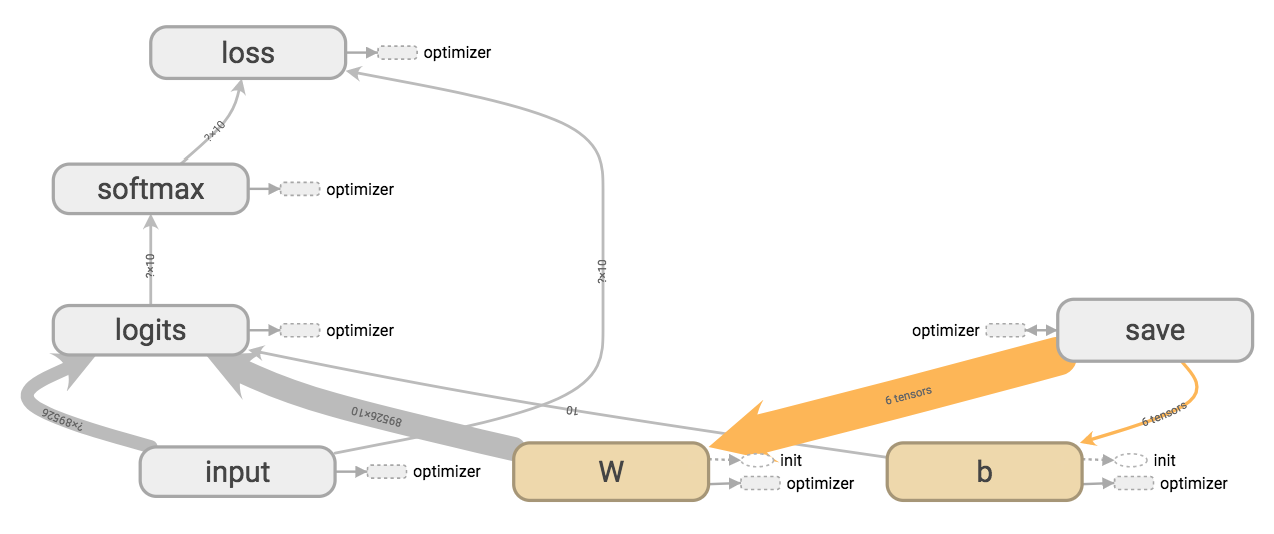
\includegraphics[width=0.8\linewidth]{figure/model_architecture}
\end{figure}
The softmax function maps each dimension of its input to a value between 0
and 1, and the transformation also normalizes the predicted probabilities such that
they sum to 1 for multi-class prediction. 

\end{block}

%----------------------------------------------------------------------------------------

\end{column} % End of column 2.1

\begin{column}{\onecolwid} % The second column within column 2 (column 2.2)

%----------------------------------------------------------------------------------------

\begin{block}{Model: LSTM}

\begin{figure}
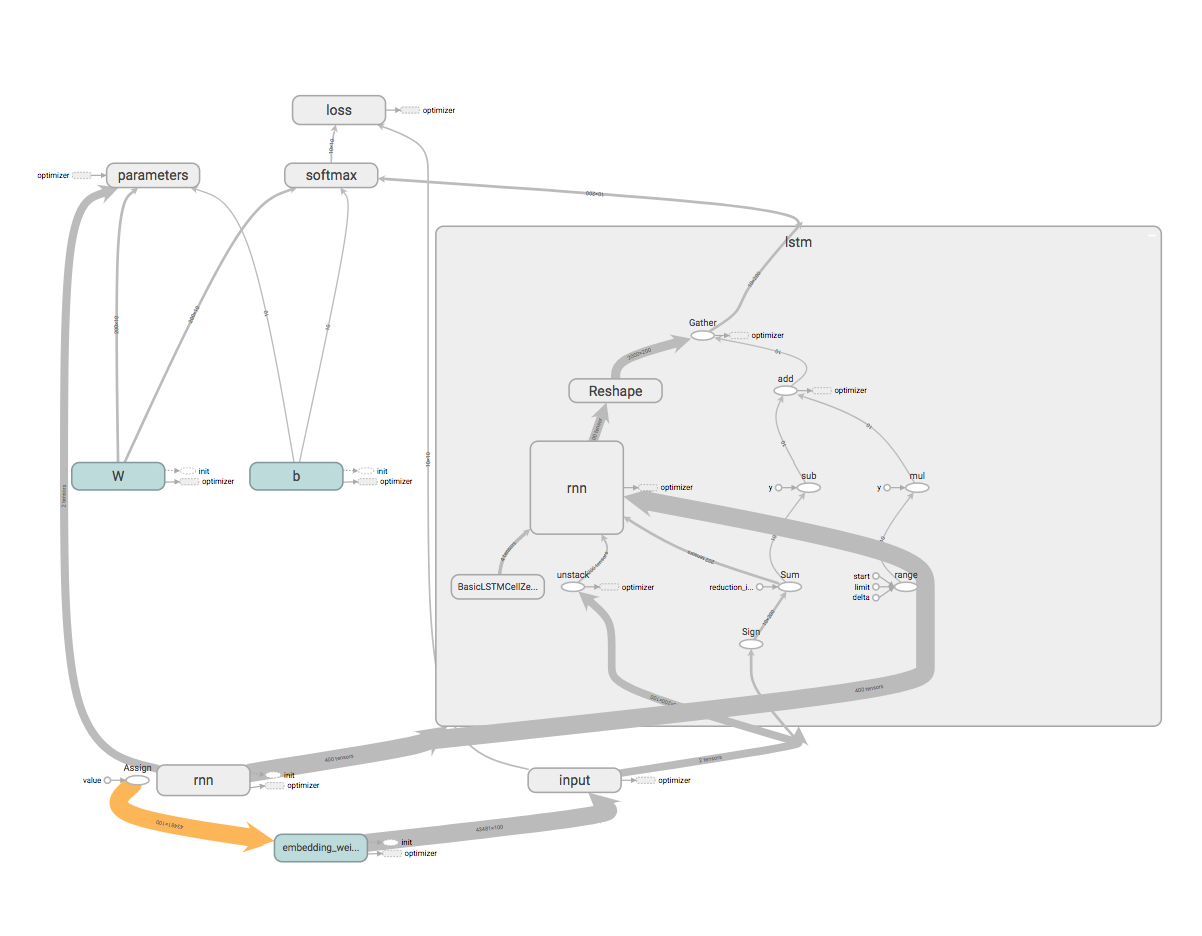
\includegraphics[width=\linewidth]{figure/lstm_architecture}
\end{figure}

\end{block}

%----------------------------------------------------------------------------------------

\end{column} % End of column 2.2

\end{columns} % End of the split of column 2

\end{column} % End of the second column

\begin{column}{\sepwid}\end{column} % Empty spacer column

\begin{column}{\onecolwid} % The third column

%----------------------------------------------------------------------------------------

\begin{block}{Model: LSTM (Cont'd)}

Given a word sequence $S=\{v_0,v_1,\ldots,v_{l-1}\}$ with length $l$, the states
of LSTM are updated as:
$$
\begin{bmatrix}
i_t\\f_t\\o_t\\c_t
\end{bmatrix} =
\begin{bmatrix}
\sigma\\\sigma\\\sigma\\\tanh
\end{bmatrix}
S[h_{t-1},x_t]
$$
\end{block}

%----------------------------------------------------------------------------------------

\begin{block}{Result}

\begin{figure}
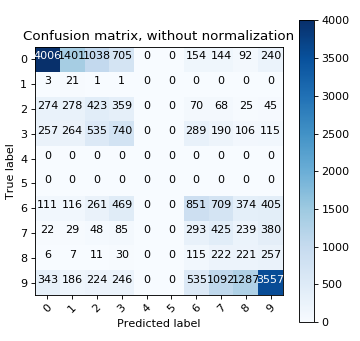
\includegraphics[width=0.8\linewidth]{figure/conf_matrix}
\end{figure}

\end{block}

%----------------------------------------------------------------------------------------

\begin{block}{Acknowledgements}

\small{\rmfamily{Project repository hosted on GitHub 
(\url{https://github.com/ufjfeng/EEL6935-Course-Project}). Web app hosted on \url{t21.ecegator.com}. All documents including this poster are written in \LaTeX}}

\begin{center}
\begin{tabular}{ccc}

\includegraphics[width=0.3\linewidth]{figure/qr_github} &  
\includegraphics[width=0.3\linewidth]{figure/qr_website} & 

\includegraphics[width=0.3\linewidth]{figure/qr_youtube}
\end{tabular}
\end{center}

\end{block}




%----------------------------------------------------------------------------------------

\end{column} % End of the third column

\end{columns} % End of all the columns in the poster

\end{frame} % End of the enclosing frame

\end{document}
